\documentclass[tikz,border=10pt]{standalone}
\usepackage{tikz}
\usepackage{amsmath,amssymb,amsfonts}
\usepackage{mathtools}
\usetikzlibrary{shapes.geometric,arrows.meta,positioning,calc,fit,backgrounds,decorations.pathmorphing}

\begin{document}
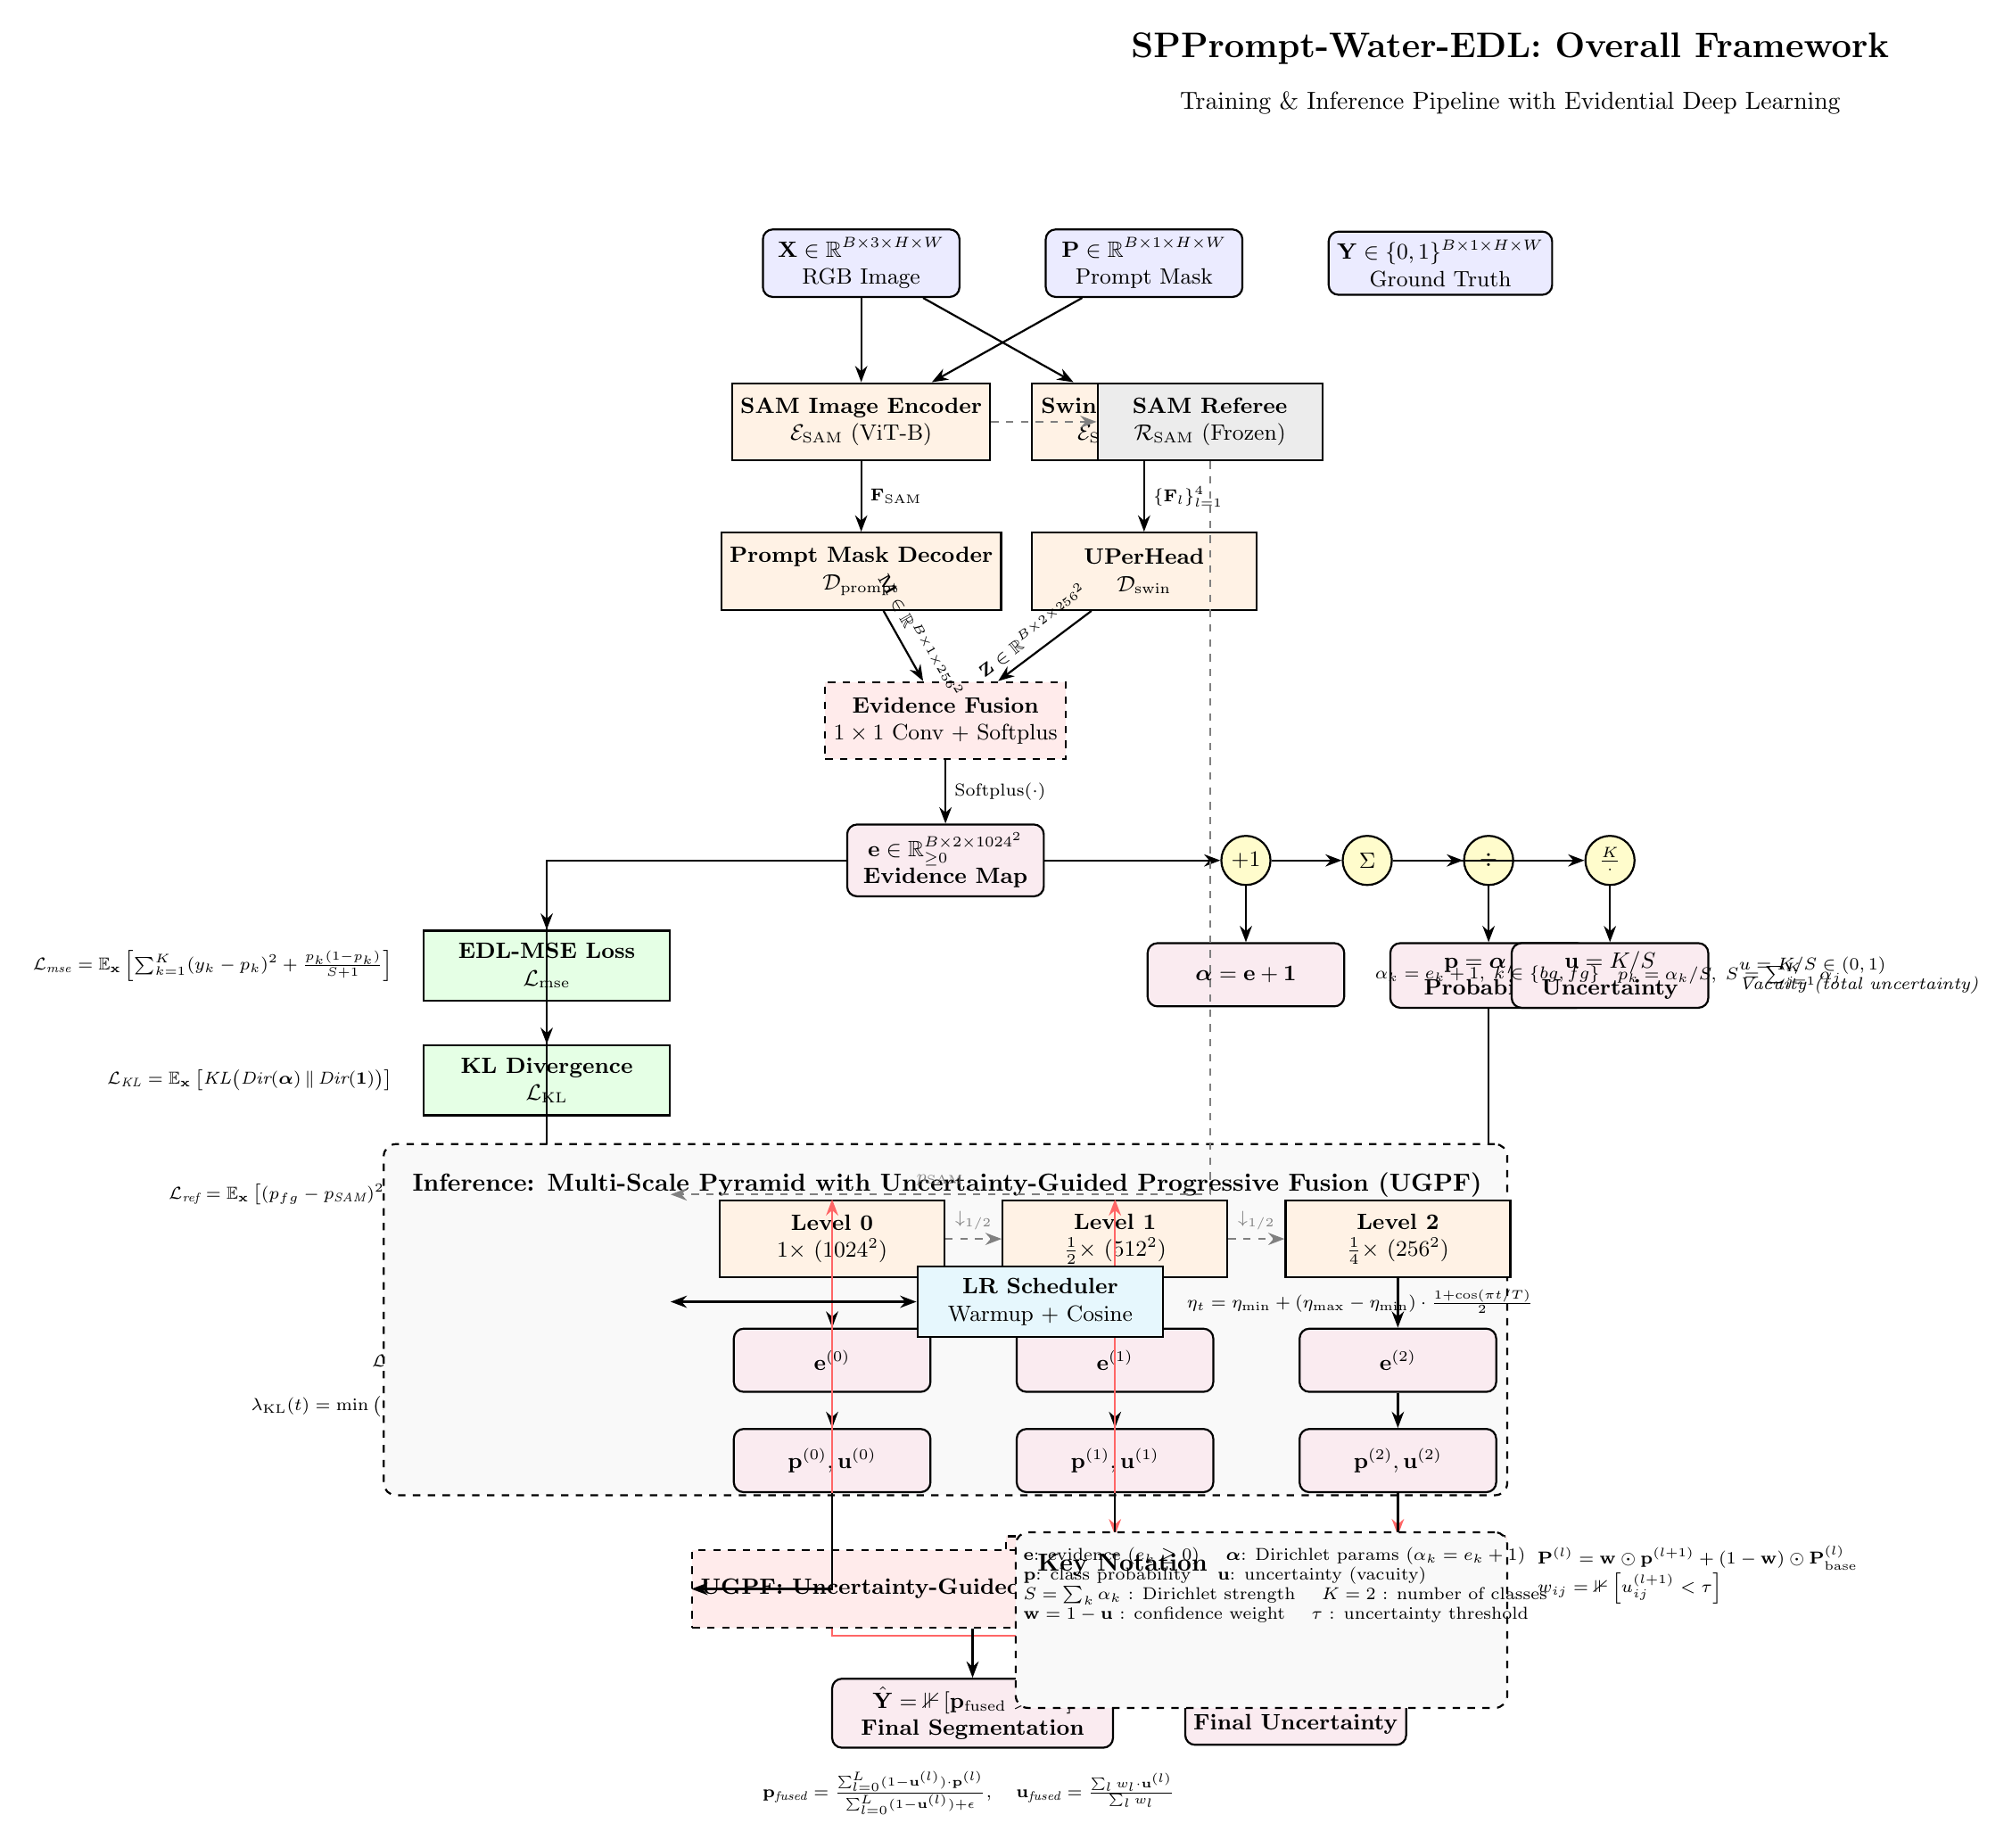
\begin{tikzpicture}[
    font=\small,
    node distance=1.2cm and 1.5cm,
    >=Stealth,
    % Node styles
    input/.style={draw,rounded corners,fill=blue!8,minimum width=2.8cm,minimum height=0.9cm,align=center,thick},
    module/.style={draw,rectangle,fill=orange!10,minimum width=3.2cm,minimum height=1.1cm,align=center,thick},
    edlmodule/.style={draw,rectangle,fill=red!8,minimum width=3.2cm,minimum height=1.1cm,align=center,thick,dashed},
    loss/.style={draw,rectangle,fill=green!10,minimum width=3.5cm,minimum height=1.0cm,align=center,thick},
    output/.style={draw,rounded corners,fill=purple!8,minimum width=2.8cm,minimum height=0.9cm,align=center,thick},
    operator/.style={draw,circle,fill=yellow!20,minimum size=0.7cm,align=center,thick,inner sep=0pt},
    arrow/.style={->,thick},
    labelbox/.style={draw=none,fill=none,align=left,font=\scriptsize\itshape},
    bigbox/.style={draw,thick,dashed,rounded corners=5pt,fill=gray!5,inner sep=8pt}
]

% ============================================================
% TITLE
% ============================================================
\node[font=\Large\bfseries] (title) at (0,12.5) {SPPrompt-Water-EDL: Overall Framework};
\node[font=\normalsize, below=0.15cm of title] (subtitle) {Training \& Inference Pipeline with Evidential Deep Learning};

% ============================================================
% SECTION 1: INPUTS
% ============================================================
\node[input, below left=1.5cm and 3cm of subtitle] (x) {$\mathbf{X} \in \mathbb{R}^{B \times 3 \times H \times W}$\\RGB Image};
\node[input, right=1.2cm of x] (p) {$\mathbf{P} \in \mathbb{R}^{B \times 1 \times H \times W}$\\Prompt Mask};
\node[input, right=1.2cm of p] (y) {$\mathbf{Y} \in \{0,1\}^{B \times 1 \times H \times W}$\\Ground Truth};

% ============================================================
% SECTION 2: ENCODER BRANCHES
% ============================================================
\node[module, below=1.2cm of x] (samenc) {\textbf{SAM Image Encoder}\\$\mathcal{E}_{\text{SAM}}$ (ViT-B)};
\node[module, below=1.2cm of p] (swin) {\textbf{Swin Transformer}\\$\mathcal{E}_{\text{SWIN}}$ (Tiny)};

\draw[arrow] (x) -- (samenc);
\draw[arrow] (x) -- (swin);
\draw[arrow] (p) -- (samenc);

% ============================================================
% SECTION 3: DECODER BRANCHES
% ============================================================
\node[module, below=1.0cm of samenc] (promptdec) {\textbf{Prompt Mask Decoder}\\$\mathcal{D}_{\text{prompt}}$};
\node[module, below=1.0cm of swin] (uper) {\textbf{UPerHead}\\$\mathcal{D}_{\text{swin}}$};

\draw[arrow] (samenc) -- node[right,font=\scriptsize] {$\mathbf{F}_{\text{SAM}}$} (promptdec);
\draw[arrow] (swin) -- node[right,font=\scriptsize] {$\{\mathbf{F}_{l}\}_{l=1}^{4}$} (uper);

% ============================================================
% SECTION 4: EVIDENCE FUSION (KEY EDL MODULE)
% ============================================================
\node[edlmodule, below=1.0cm of promptdec, xshift=1.2cm] (fusion) {\textbf{Evidence Fusion}\\$1\times1$ Conv + Softplus};

\draw[arrow] (promptdec) -- node[above,sloped,font=\scriptsize] {$\mathbf{M} \in \mathbb{R}^{B \times 1 \times 256^2}$} (fusion);
\draw[arrow] (uper) -- node[above,sloped,font=\scriptsize] {$\mathbf{Z} \in \mathbb{R}^{B \times 2 \times 256^2}$} (fusion);

% ============================================================
% EVIDENCE OUTPUT
% ============================================================
\node[output, below=0.9cm of fusion] (evidence) {$\mathbf{e} \in \mathbb{R}_{\geq 0}^{B \times 2 \times 1024^2}$\\\textbf{Evidence Map}};
\draw[arrow] (fusion) -- node[right,font=\scriptsize] {$\text{Softplus}(\cdot)$} (evidence);

% ============================================================
% DIRICHLET CONVERSION (RIGHT SIDE)
% ============================================================
\node[operator, right=2.5cm of evidence] (alpha) {$+1$};
\node[operator, right=1.0cm of alpha] (sum) {$\Sigma$};
\node[operator, right=1.0cm of sum] (div) {$\div$};
\node[operator, right=1.0cm of div] (kdiv) {$\frac{K}{\cdot}$};

\node[output, below=0.8cm of alpha] (alphaout) {$\boldsymbol{\alpha} = \mathbf{e} + \mathbf{1}$};
\node[output, below=0.8cm of div] (prob) {$\mathbf{p} = \boldsymbol{\alpha} / S$\\\textbf{Probability}};
\node[output, below=0.8cm of kdiv] (unc) {$\mathbf{u} = K / S$\\\textbf{Uncertainty}};

\draw[arrow] (evidence) -- (alpha);
\draw[arrow] (alpha) -- (sum);
\draw[arrow] (sum) -- (div);
\draw[arrow] (sum) -- (kdiv);
\draw[arrow] (alpha) -- (alphaout);
\draw[arrow] (div) -- (prob);
\draw[arrow] (kdiv) -- (unc);

% Formulas
\node[labelbox, right=0.3cm of alphaout] (alphalabel) {$\alpha_k = e_k + 1,\; k \in \{bg, fg\}$};
\node[labelbox, right=0.3cm of prob] (plabel) {$p_k = \alpha_k / S,\; S = \sum_{j=1}^{K} \alpha_j$};
\node[labelbox, right=0.3cm of unc] (ulabel) {$u = K / S \in (0,1)$\\Vacuity (total uncertainty)};

% ============================================================
% LOSS FUNCTIONS (LEFT SIDE)
% ============================================================
\node[loss, left=2.5cm of evidence, yshift=-1.5cm] (mse) {\textbf{EDL-MSE Loss}\\$\mathcal{L}_{\text{mse}}$};
\node[loss, below=0.6cm of mse] (kl) {\textbf{KL Divergence}\\$\mathcal{L}_{\text{KL}}$};
\node[loss, below=0.6cm of kl] (ref) {\textbf{Referee Loss}\\$\mathcal{L}_{\text{ref}}$};

\draw[arrow] (evidence) -| (mse);
\draw[arrow] (evidence) -| (kl);
\draw[arrow] (prob) |- (ref);

% Loss formulas
\node[labelbox, left=0.2cm of mse, align=right] (mselabel) {
    $\mathcal{L}_{\text{mse}} = \mathbb{E}_{\mathbf{x}}\left[\sum_{k=1}^{K}(y_k - p_k)^2 + \frac{p_k(1-p_k)}{S+1}\right]$
};
\node[labelbox, left=0.2cm of kl, align=right] (kllabel) {
    $\mathcal{L}_{\text{KL}} = \mathbb{E}_{\mathbf{x}}\left[\text{KL}\big(\text{Dir}(\boldsymbol{\alpha}) \,\|\, \text{Dir}(\mathbf{1})\big)\right]$
};
\node[labelbox, left=0.2cm of ref, align=right] (reflabel) {
    $\mathcal{L}_{\text{ref}} = \mathbb{E}_{\mathbf{x}}\left[(p_{fg} - p_{\text{SAM}})^2\right]$
};

% ============================================================
% TOTAL LOSS
% ============================================================
\node[loss, below=0.5cm of ref, xshift=0cm, fill=green!25] (totalloss) {\textbf{Total Loss}\\$\mathcal{L}_{\text{total}}$};

\draw[arrow] (mse) -- (totalloss);
\draw[arrow] (kl) -- (totalloss);
\draw[arrow] (ref) -- (totalloss);

\node[labelbox, below=0.1cm of totalloss, align=center] (totallabel) {
    $\mathcal{L}_{\text{total}} = \mathcal{L}_{\text{mse}} + \lambda_{\text{KL}}(t) \cdot \mathcal{L}_{\text{KL}} + w_{\text{ref}} \cdot \mathcal{L}_{\text{ref}}$
};

% Annealing formula
\node[labelbox, below=0.1cm of totallabel, align=center, font=\scriptsize] (annelabel) {
    $\lambda_{\text{KL}}(t) = \min\left(1,\; \frac{t}{T \cdot r}\right),\; t: \text{epoch},\; T: \text{total epochs},\; r: \text{anneal ratio}$
};

% ============================================================
% INFERENCE: PYRAMID + UGPF (BOTTOM)
% ============================================================
\node[bigbox, below=3.5cm of evidence, minimum width=16cm, minimum height=5cm] (infbox) {};
\node[font=\bfseries, anchor=north west] at ($(infbox.north west)+(0.3,-0.3)$) {Inference: Multi-Scale Pyramid with Uncertainty-Guided Progressive Fusion (UGPF)};

% Pyramid levels
\node[module, below left=0.8cm and 0cm of infbox.north] (l0) {\textbf{Level 0}\\$1\times$ (1024$^2$)};
\node[module, right=0.8cm of l0] (l1) {\textbf{Level 1}\\$\frac{1}{2}\times$ (512$^2$)};
\node[module, right=0.8cm of l1] (l2) {\textbf{Level 2}\\$\frac{1}{4}\times$ (256$^2$)};

% Down arrows
\draw[arrow, dashed, gray] (l0) -- node[above,font=\scriptsize] {$\downarrow_{1/2}$} (l1);
\draw[arrow, dashed, gray] (l1) -- node[above,font=\scriptsize] {$\downarrow_{1/2}$} (l2);

% Evidence outputs per level
\node[output, below=0.7cm of l0] (e0) {$\mathbf{e}^{(0)}$};
\node[output, below=0.7cm of l1] (e1) {$\mathbf{e}^{(1)}$};
\node[output, below=0.7cm of l2] (e2) {$\mathbf{e}^{(2)}$};

\draw[arrow] (l0) -- (e0);
\draw[arrow] (l1) -- (e1);
\draw[arrow] (l2) -- (e2);

% Prob/Unc per level
\node[output, below=0.5cm of e0] (p0) {$\mathbf{p}^{(0)}, \mathbf{u}^{(0)}$};
\node[output, below=0.5cm of e1] (p1) {$\mathbf{p}^{(1)}, \mathbf{u}^{(1)}$};
\node[output, below=0.5cm of e2] (p2) {$\mathbf{p}^{(2)}, \mathbf{u}^{(2)}$};

\draw[arrow] (e0) -- (p0);
\draw[arrow] (e1) -- (p1);
\draw[arrow] (e2) -- (p2);

% Uncertainty-Gated Prompt Propagation (top-down)
\node[edlmodule, below=0.6cm of p2, minimum width=3cm] (gate2) {\textbf{Uncertainty Gate}\\$\mathbf{u}^{(2)} < \tau$?};
\node[edlmodule, below=0.6cm of p1, minimum width=3cm] (gate1) {\textbf{Uncertainty Gate}\\$\mathbf{u}^{(1)} < \tau$?};

\draw[arrow, thick, red!60] (p2) -- (gate2);
\draw[arrow, thick, red!60] (gate2.south) |- ++(0,-0.3) -| (l1.north);
\draw[arrow, thick, red!60] (p1) -- (gate1);
\draw[arrow, thick, red!60] (gate1.south) |- ++(0,-0.3) -| (l0.north);

% Gate formulas
\node[labelbox, right=0.3cm of gate2, font=\scriptsize] (gatelabel) {
    $\mathbf{P}^{(l)} = \mathbf{w} \odot \mathbf{p}^{(l+1)} + (1-\mathbf{w}) \odot \mathbf{P}_{\text{base}}^{(l)}$\\
    $w_{ij} = \mathbb{1}\left[u_{ij}^{(l+1)} < \tau\right]$
};

% UGPF Fusion
\node[edlmodule, below=0.8cm of p0, xshift=2cm, minimum width=5cm] (ugpf) {\textbf{UGPF: Uncertainty-Guided Progressive Fusion}};

\draw[arrow] (p0) |- (ugpf);
\draw[arrow] (p1) |- (ugpf);
\draw[arrow] (p2) |- (ugpf);

% Final output
\node[output, below=0.7cm of ugpf, minimum width=4cm] (final) {$\hat{\mathbf{Y}} = \mathbb{1}\left[\mathbf{p}_{\text{fused}} > 0.5\right]$\\\textbf{Final Segmentation}};
\node[output, right=1.0cm of final] (finalunc) {$\mathbf{u}_{\text{fused}}$\\\textbf{Final Uncertainty}};

\draw[arrow] (ugpf) -- (final);
\draw[arrow] (ugpf) -- (finalunc);

% UGPF formula
\node[labelbox, below=0.2cm of final, align=center] (ugpflabel) {
    $\mathbf{p}_{\text{fused}} = \frac{\sum_{l=0}^{L} (1 - \mathbf{u}^{(l)}) \cdot \mathbf{p}^{(l)}}{\sum_{l=0}^{L} (1 - \mathbf{u}^{(l)}) + \epsilon},\quad \mathbf{u}_{\text{fused}} = \frac{\sum_{l} w_l \cdot \mathbf{u}^{(l)}}{\sum_{l} w_l}$
};

% ============================================================
% SAM REFEREE BRANCH (SIDE)
% ============================================================
\node[module, right=1.5cm of samenc, fill=gray!15] (referee) {\textbf{SAM Referee}\\$\mathcal{R}_{\text{SAM}}$ (Frozen)};
\draw[arrow, dashed, gray] (samenc) -- (referee);
\draw[arrow, dashed, gray] (referee) |- node[near end,above,font=\scriptsize] {$p_{\text{SAM}}$} (ref);

% ============================================================
% TRAINING SCHEDULER
% ============================================================
\node[loss, right=3.5cm of totalloss, fill=cyan!10] (sched) {\textbf{LR Scheduler}\\Warmup + Cosine};
\draw[arrow, <->] (totalloss) -- (sched);
\node[labelbox, right=0.2cm of sched, align=left] (schedlabel) {
    $\eta_t = \eta_{\min} + (\eta_{\max} - \eta_{\min}) \cdot \frac{1 + \cos(\pi t / T)}{2}$
};

% ============================================================
% NOTATION LEGEND
% ============================================================
\node[bigbox, below left=0.5cm and 0cm of infbox.south east, minimum width=7cm, minimum height=2.5cm, anchor=north east] (legend) {};
\node[font=\bfseries, anchor=north west] at ($(legend.north west)+(0.2,-0.2)$) {Key Notation};
\node[labelbox, below=0.1cm of legend.north west, anchor=north west, font=\scriptsize] (legtext) {
    $\mathbf{e}$: evidence ($e_k \geq 0$) \quad $\boldsymbol{\alpha}$: Dirichlet params ($\alpha_k = e_k + 1$)\\
    $\mathbf{p}$: class probability \quad $\mathbf{u}$: uncertainty (vacuity)\\
    $S = \sum_k \alpha_k$ : Dirichlet strength \quad $K=2$ : number of classes\\
    $\mathbf{w} = 1 - \mathbf{u}$ : confidence weight \quad $\tau$ : uncertainty threshold
};

\end{tikzpicture}
\end{document}
